\documentclass[10pt]{article}

\usepackage{adjustbox}
\usepackage{amsmath}
\usepackage{amssymb}
\usepackage[spanish]{babel}
\usepackage{fancyhdr}
\usepackage{float}
\usepackage[T1]{fontenc}
\usepackage{graphicx}
\usepackage[utf8]{inputenc}
\usepackage{mathtools}
\usepackage{multicol}
\usepackage{multirow}
\usepackage{wasysym}
\usepackage[svgnames]{xcolor}
\usepackage[paperheight=27.94cm,paperwidth=21.59cm,left=2.54cm,right=2.54cm,top=2.54cm,bottom=2.54cm]{geometry}


\setlength\parindent{0pt}
\renewcommand{\arraystretch}{1.3}\lfoot{\thepage}



\title{FACULTAD DE INGENIERÍA Y CIENCIAS}
\author{Cristóbal Fajardo, Pablo Gaete, Rubén Torres \\ 
Profesor Guía: Juan Bekios}
\begin{document}
\maketitle

\vspace{5\baselineskip}
\begin{center}
{\Large \textbf{COMBINANDO VISIÓN ARTIFICIAL Y MODELOS DE LENGUAJE PARA INTERPRETACIÓN DE LENGUA DE SEÑAS CHILENA (LSCh)}\par}
\end{center}

\vspace{5\baselineskip}



\vspace{1\baselineskip}
\begin{center}
{\large Cristóbal Fajardo, Pablo Gaete, Rubén Torres}
\end{center}


\begin{center}
{\large Profesor guía: Juan Bekios Calfa}
\end{center}


\vspace{5\baselineskip}
\begin{center}
{\small SANTIAGO-CHILE 2024}
\end{center}


\vspace{3\baselineskip}
\newpage
\begin{center}
{\Large\textbf{Resumen}}
\end{center}

\vspace{1\baselineskip}
La escasez de intérpretes de Lengua de Señas Chilena (LSCh), especialmente en el ámbito de la salud, representa un desafío significativo para las personas sordas en Chile, dificultando el acceso a un tratamiento adecuado particularmente en el área de la salud mental. En este trabajo, se propone una solución digital que ofrece una alternativa accesible y de menor costo en comparación con los intérpretes profesionales. Nuestra propuesta combina la detección de puntos clave de las manos (hand landmark detection) con redes neuronales LSTM, complementadas por un modelo de lenguaje de gran escala (LLM) para lograr una mayor fluidez al transformar señas individuales en oraciones completa.

El sistema ha demostrado una tasa de acierto del 92.5$\%$ en el reconocimiento de palabras individuales y una similitud del 96.35$\%$ comparado con las frases esperadas (utilizando la distancia de Levenshtein) en la traducción de frases completas. Además, utiliza una arquitectura cliente-servidor, que asegura escalabilidad y accesibilidad desde dispositivos con recursos limitados. A pesar de estos resultados prometedores, áreas como la ampliación del dataset y la reducción de latencia siguen siendo desafíos clave para el desarrollo futuro.

Esta solución digital no solo tiene el potencial de mejorar el acceso de las personas sordas en Chile a servicios críticos, sino que también abre nuevas oportunidades para la investigación y el desarrollo de tecnologías inclusivas en el ámbito de la comunicación asistida.

\vspace{1\baselineskip}
\section{Introducción}

\subsection{Descripción del problema}

En Chile, el II Estudio Nacional de la Discapacidad realizado por el Ministerio de Desarrollo Social y SENADIS en 2015 , el 16,7$\%$ de la población presenta algún tipo de discapacidad, equivalente a 2.836.818 personas. De estas, el 3,6$\%$ tiene dificultades auditivas, lo que representa aproximadamente 611.000 personas, de las cuales 180.000 padecen sordera total .

La escasez de intérpretes de Lengua de Señas genera una significativa exclusión de las personas sordas en nuestra sociedad, una situación particularmente evidente en el ámbito de la salud, uno de los pilares fundamentales para el bienestar humano.

En el ámbito de la salud mental, las personas sordas enfrentan una exclusión sistemática debido a la falta de comunicación efectiva con los profesionales, lo que incrementa los riesgos de exclusión social y dificulta su bienestar. Esta problemática resalta la necesidad urgente de soluciones tecnológicas que puedan abordar estas brechas de accesibilidad.

\subsection{Hipótesis de trabajo}

\vspace{1\baselineskip}
La implementación de un modelo de interpretación del Lenguaje de Señas Chileno (LSCh)

utilizando detección de manos con landmarks y redes neuronales LSTM, combinado con un

modelo de lenguaje (LLM) puede alcanzar una tasa de acierto mayor al 90$\%$, con un costo menor y una disponibilidad mayor que un intérprete humano.

\vspace{1\baselineskip}
\subsection{Objetivos}

\subsubsection{General}

Diseñar e implementar un sistema automatizado que interprete LSCh mediante visión artificial y procesamiento de lenguaje natural, para mejorar el acceso a servicios de salud por parte de personas sordas.

\subsubsection{Específicos}

\begin{enumerate}
	\item Investigar tecnologías avanzadas aplicadas al reconocimiento de lenguas de señas, incluyendo visión artificial y modelos de lenguaje.

	\item Implementar un modelo que integre MediaPipe para la detección de landmarks, LSTM para el análisis secuencial y LLM para la generación de traducciones coherentes.

	\item Evaluar la efectividad del sistema mediante métricas como precisión, similitud textual y latencia.

\end{enumerate}
\vspace{1\baselineskip}
\section{Estado del Arte}

\subsection{Discusión bibliográfica}

El reconocimiento de la Lengua de Señas Chilena (LSCh) ha sido un desafío técnico y social abordado en diversas investigaciones. Los primeros enfoques, como los modelos basados en Support Vector Machines (SVM), que corresponden a un conjunto de algoritmos de aprendizaje estadístico supervisado pertenecientes a la familia de los clasificadores lineales desarrollados por Vladimir Vapnik en torno al año 1995. Una SVM construye un hiperplano en un espacio de dimensionalidad muy alta y separa de forma óptima los puntos de una clase de la de otra. En el concepto de ``separación óptima" es donde reside la característica fundamental de las SVM, se busca el hiperplano que tenga la máxima distancia (margen) con los puntos que estén más cerca de él mismo. Entre sus aplicaciones se encuentra el reconocimiento de email spam, escritura a mano y clasificación de imágenes.

\vspace{1\baselineskip}
Su implementación logró altos niveles de aciertos en ambientes controlados, alcanzando un 100$\%$ en alfabetos visuales estáticos. Sin embargo, su desempeño disminuye significativamente en entornos no controlados, con aciertos de hasta un 80$\%$ .

\vspace{1\baselineskip}
Este enfoque tiene algunas ventajas, como el uso eficiente de memoria, lo cual permite ser ejecutado en un dispositivo móvil Android. Sin embargo su principal limitación es que sólo puede identificar gestos estáticos, pero no secuencias de gestos, las cuales son necesarias para expresar muchos conceptos y oraciones . Otra limitación consiste en la falta de flexibilidad para funcionar bien en condiciones no ideales, por ejemplo, cuando la iluminación no es la más óptima.

\vspace{1\baselineskip}
Un enfoque más robusto es el modelo YOLO-v9e (You Only Look Once), una red neuronal convolucional diseñada específicamente para la detección de objetos en tiempo real. Este modelo, aplicado a la identificación de gestos que representan caracteres individuales del alfabeto, ha demostrado ser altamente efectivo  en conjuntos de datos de la Lengua de Señas Norteamericana (ASL) . YOLO-v9e, optimizada para estos escenarios, reportó una precisión del 96.83$\%$, un recall del 92.96$\%$, y un mAP@0.5 del 97.84$\%$, validando su capacidad para reconocer gestos con alta precisión en aplicaciones prácticas  Sin embargo, éste presenta limitaciones para procesar secuencias, además requiere un gran volumen de datos etiquetados con precisión para cada gesto. En cual no está disponible en el caso de la LSCh. 

\vspace{1\baselineskip}
Ambos acercamientos tienen en común su factibilidad de ejecución en un dispositivo móvil, para permitir la portabilidad. Esta limitación la podemos superar al utilizar una arquitectura cliente-servidor que permita ejecutar el modelo de detección de las señas en un servidor con mayor capacidad computacional, y visualizar el resultado en un dispositivo móvil a través de una conexión a internet.

\vspace{1\baselineskip}
Un avance importante en la interpretación de gestos secuenciales lo representan las redes convolucionales tridimensionales (3D-CNN) han mostrado ser capaces de procesar gestos secuenciales al modelar características espacio-temporales. Estas redes ofrecen una alta precisión para interpretar secuencias complejas, pero requieren altos recursos computacionales y grandes datasets etiquetados, lo que las hace menos viables para aplicaciones en lenguas de señas con recursos limitados .

\vspace{1\baselineskip}
Una forma eficiente de simplificar los datos de entrada del modelo es mediante la utilización de un sistema de landmarks, que sintetiza la información relevante en una serie de puntos clave, como las articulaciones y las puntas de los dedos. Estos landmarks actúan como una representación estructurada y compacta de los gestos, eliminando información redundante y preservando las características esenciales del movimiento. Este enfoque no solo optimiza el procesamiento de datos al reducir la complejidad del modelo, sino que también mejora la precisión en la identificación de gestos al proporcionar un conjunto consistente de referencias visuales que representan los movimientos de las manos de manera precisa .

\vspace{1\baselineskip}
Una vez superado el reto de identificar secuencias de gestos, permanece el reto de traducir al castellano de forma fluida y coherente. Un acercamiento que puede ser beneficioso en esta etapa, es la integración de un LLM. 

\vspace{1\baselineskip}
Los Modelos de Lenguaje de Gran Escala permiten interpretar variaciones en las señas dentro del contexto de frases completas, ofreciendo traducciones más precisas y coherentes que trascienden la mera clasificación de gestos individuales. El método SignLLM, basado en este enfoque, fue evaluado en los conjuntos de datos PHOENIX-2014T (lengua de señas alemana) y CSL-Daily (lengua de señas china), logrando resultados destacados. En PHOENIX-2014T, el modelo alcanzó una puntuación BLEU-4 de 25.25 en el conjunto de validación y 23.40 en el de prueba, mientras que en CSL-Daily obtuvo 12.23 y 15.75, respectivamente. Además, las puntuaciones ROUGE, que evalúan la recuperación del contenido clave, fueron de 47.23 (validación) y 44.49 (prueba) en PHOENIX-2014T, y de 39.18 (validación) y 39.91 (prueba) en CSL-Daily. Estas métricas demuestran que SignLLM logra mantener un equilibrio entre la precisión gramatical y la coherencia semántica, destacando su efectividad en comparación con otros métodos gloss-free que no utilizan glosas.

\subsection{Marco Teórico}

El marco teórico aborda las tecnologías clave que sustentan la interpretación automatizada de la Lengua de Señas Chilena (LSCh), incluyendo MediaPipe, redes LSTM, modelos de lenguaje natural (LLM), métricas de evaluación y una arquitectura cliente-servidor, que veremos a continuación, fundamentales para garantizar la precisión y eficiencia del sistema.

\subsubsection{MediaPipe y Procesamiento de Gestos}

MediaPipe es una herramienta de visión artificial que permite la detección en tiempo real de landmarks o puntos clave en las manos, como articulaciones y puntas de los dedos. Su diseño eficiente lo hace adecuado para dispositivos con recursos computacionales limitados, proporcionando datos estructurados que facilitan el análisis de gestos. 

\begin{figure}[H]
\centering
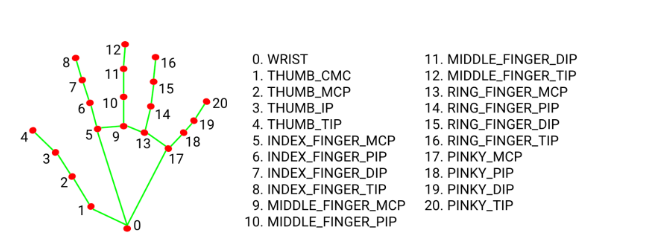
\includegraphics[width=14.33cm,height=5.46cm]{./images/image4.png}
\end{figure}


\vspace{1\baselineskip}
\begin{center}
\textit{Figura 1. Hand landmarks de MediaPipe}
\end{center}


\subsubsection{Procesamiento Secuencial: Redes LSTM}

Las redes LSTM (Long Short-Term Memory) son una variante de redes neuronales recurrentes diseñadas para modelar secuencias temporales y resolver problemas de aprendizaje a largo plazo. Utilizan tres puertas: olvido, entrada y salida, para controlar el flujo de información, permitiendo conservar información relevante y descartar datos innecesarios.

\vspace{1\baselineskip}
\begin{figure}[H]
\centering
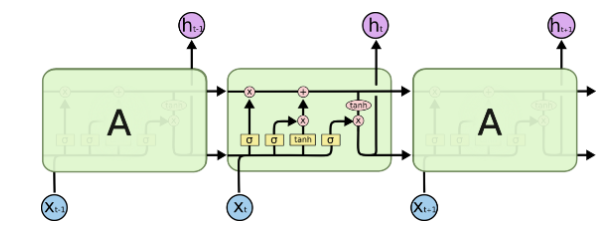
\includegraphics[width=10.0cm,height=3.79cm]{./images/image6.png}
\end{figure}


\begin{center}
\ \ \ \ \textit{Figura 2. }módulo de repetición en un LSTM
\end{center}


\vspace{2\baselineskip}
\subsubsection{Adam (Adaptive Moment Estimation)}

Algoritmo de optimización que ajusta dinámicamente las tasas de aprendizaje utilizando promedios móviles de gradientes y sus cuadrados para mejorar la eficiencia del entrenamiento.

\subsubsection{Early Stopping}

Early Stopping es una técnica de regularización que monitorea el rendimiento de un modelo en un conjunto de validación durante el entrenamiento. Su objetivo es identificar el momento óptimo para detener el entrenamiento antes de que el modelo comience a sobre ajustarse a los datos de entrenamiento. 

\vspace{1\baselineskip}
\begin{figure}[H]
\centering
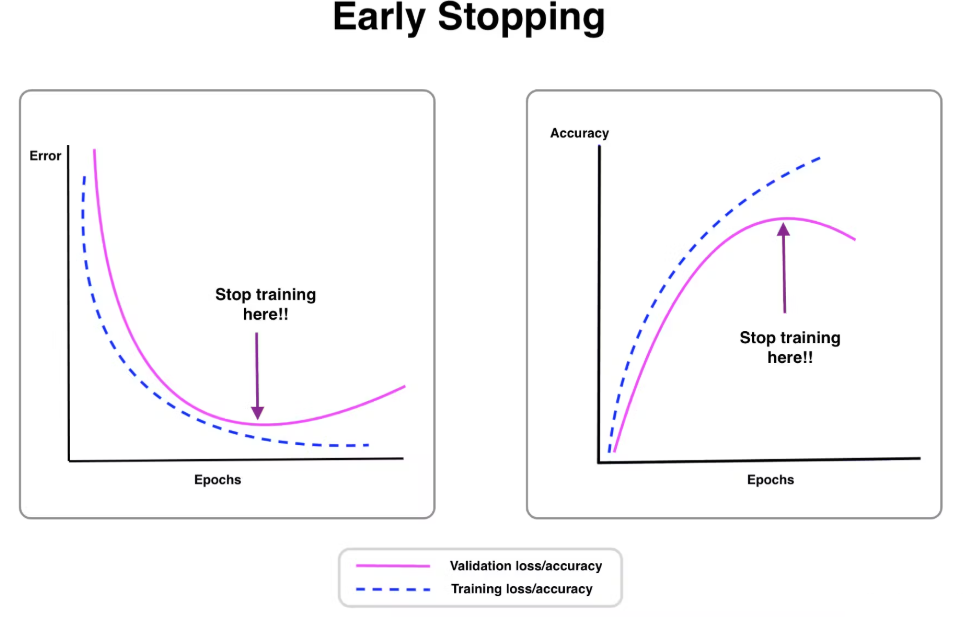
\includegraphics[width=8.7cm,height=5.54cm]{./images/image2.png}
\end{figure}


\begin{center}
\textit{Figura 3. }Grafico Early Stopping
\end{center}


\subsubsection{Modelos de Lenguaje Natural: LLM}

Los modelos de lenguaje de gran escala son sistemas entrenados en grandes corpus textuales para generar texto coherente y contextualizado. Estos modelos incorporan el contexto semántico de las palabras, lo que les permite producir traducciones fluidas y adaptadas a estructuras gramaticales complejas.

\vspace{1\baselineskip}
\begin{figure}[H]
\centering
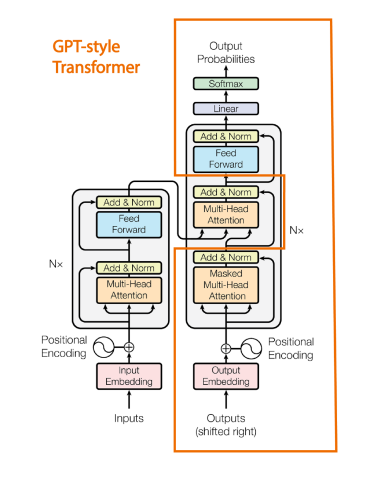
\includegraphics[width=6.6cm,height=8.14cm]{./images/image1.png}
\end{figure}


\begin{center}
\textit{Figura 4. Esquema de modelo transformer como gpt-4o mini}
\end{center}


\subsubsection{Métricas de Evaluación}

En este proyecto, se utilizaron métricas clave para evaluar el desempeño del modelo en las tareas de clasificación y traducción, garantizando resultados precisos y relevantes. Estas métricas en conjunto ofrecen una visión integral del desempeño del modelo, abarcando tanto el nivel de predicciones individuales como la calidad semántica de las frases completas.

\paragraph{Precisión (Accuracy)}

La precisión mide el porcentaje de predicciones correctas realizadas por el modelo, considerando tanto las clases positivas como negativas. Se define como:

\vspace{1\baselineskip}
\( Accuracy(correct classifications / total classifications) =  TP+TN / TP+TN+FP+FN\)\ \ \ \ \ \ \ 

\vspace{1\baselineskip}
\begin{flushleft}
Donde TP (True Positives) representa los verdaderos positivos, TN (True Negatives) los verdaderos negativos, FP (False Positives) los falsos positivos, y FN (False Negatives) los falsos negativos. Esta métrica proporciona una visión general del rendimiento global del modelo, aunque puede no ser adecuada en escenarios con conjuntos de datos desbalanceados.
\end{flushleft}


\paragraph{Función de Pérdida Categorical Crossentropy}

La categorical crossentropy mide la discrepancia entre las distribuciones predicha y real en problemas de clasificación multiclase. Matemáticamente, se define como:

\vspace{1\baselineskip}
\( H(p, q)  =  -\sum_{rex}^{}p(x)log(q(x))\)\ \ \ \ \ \ 

\vspace{1\baselineskip}
\begin{flushleft}
Donde p(x) representa la distribución real y q(x) la predicción del modelo para cada clase x. Esta función penaliza más las predicciones incorrectas que las correctas, incentivando al modelo a aprender distribuciones precisas para cada clase. \ \ \ \ \ \ \ 
\end{flushleft}


\paragraph{Distancia de Levenshtein}

La distancia de Levenshtein evalúa la similitud entre cadenas de texto, calculando el número mínimo de operaciones (inserciones, eliminaciones o sustituciones) necesarias para transformar una cadena en otra. La métrica empleada es:

\vspace{1\baselineskip}
\( P  =  (1 -levenshtein(E, A) / max(len(E), len(A)) \ast  100\)

\vspace{1\baselineskip}
\begin{flushleft}
Donde E representa la cadena esperada, A la cadena predicha, levenshtein(E,A) es la distancia de Levenshtein entre E y A, len() indica la longitud de una cadena. Esta métrica es fundamental para evaluar traducciones textuales, ya que mide la precisión con la que las frases predichas se corresponden con las esperadas.
\end{flushleft}


\subsubsection{Arquitectura Cliente-Servidor}

La arquitectura cliente-servidor es un modelo de diseño computacional que distribuye tareas entre un cliente (dispositivo del usuario) y un servidor centralizado. El cliente captura y envía datos al servidor, que los procesa utilizando modelos de inteligencia artificial y devuelve los resultados. Este diseño garantiza la escalabilidad y optimiza los recursos, permitiendo que el cliente realice operaciones ligeras mientras el servidor asume la carga computacional más intensiva.

\subsubsection{Arquitectura de YOLO-v9e}

YOLO-v9e está optimizado para la detección de objetos en tiempo real mediante tres componentes clave: Backbone, que extrae características iniciales; Neck, que refina estas características para detección multi-escala; y Head, que predice cajas delimitadoras y probabilidades de clase para objetos de distintos tamaños.

\vspace{1\baselineskip}
Un elemento crucial es la fórmula de Confidence Score, que evalúa la calidad de las predicciones:

\( Confidence (C)  =  P(Object) X IoUtruth, pred\)

Aquí, (Object) representa la probabilidad de que haya un objeto en la caja predicha, mientras que IoUtruth mide la superposición entre la caja predicha y la caja verdadera. 

\vspace{1\baselineskip}
\begin{center}
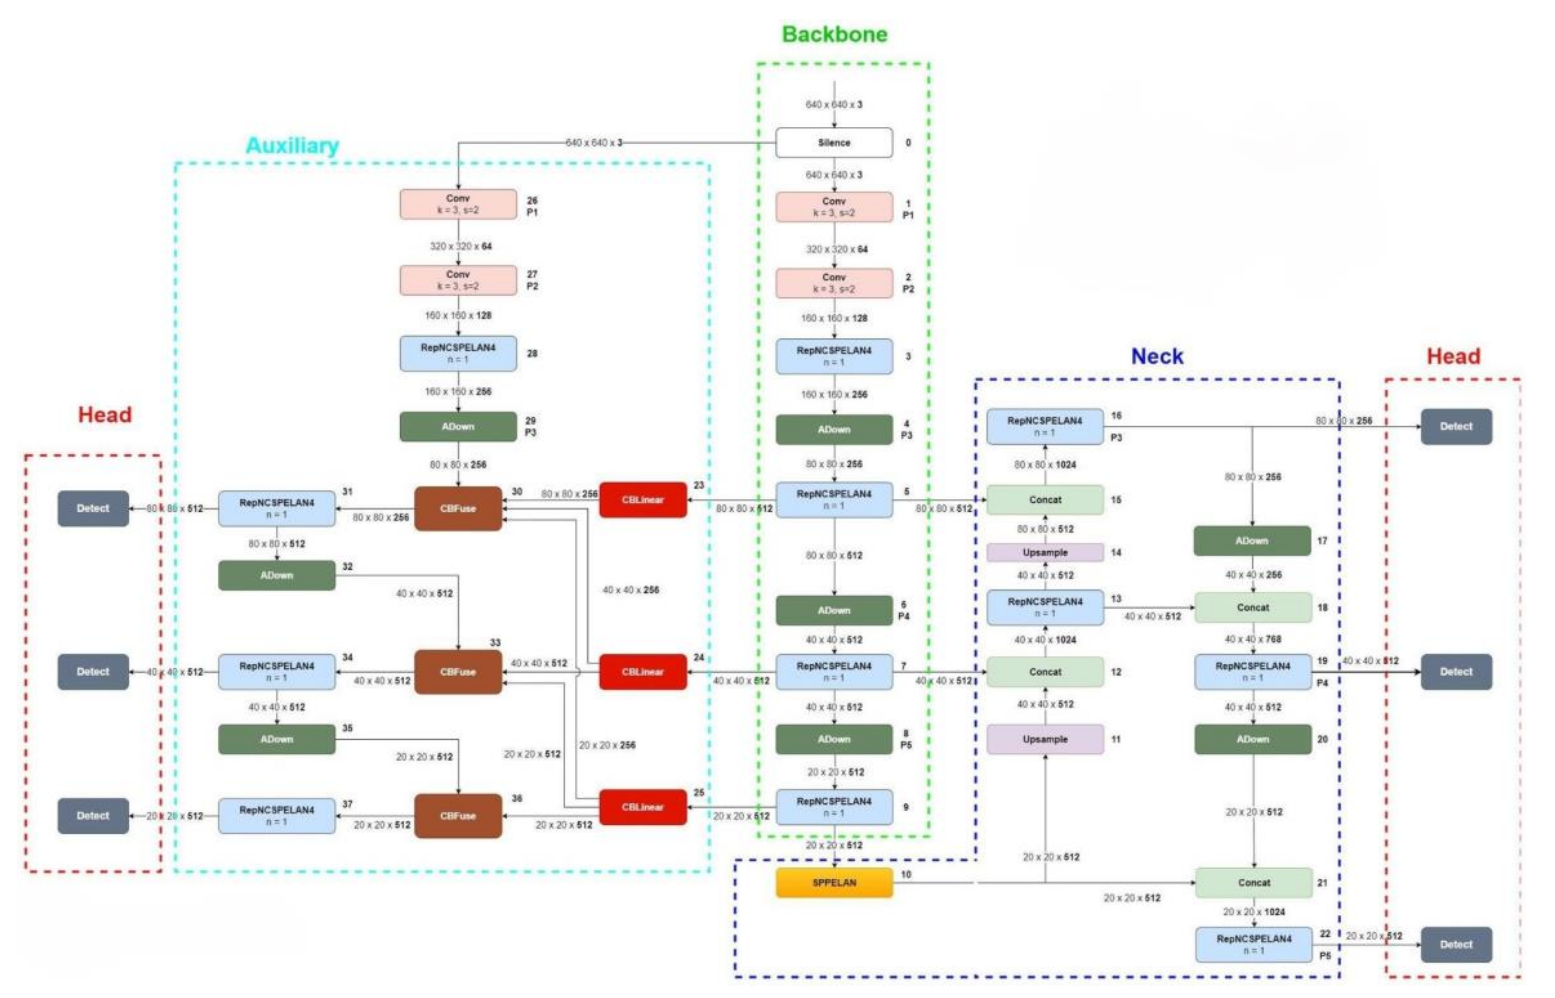
\includegraphics[width=16.51cm,height=10.58cm]{./images/image5.png}
\textit{Figura 5. Arquitectura de Funcionamiento del Modelo YOLO-v9e}
\end{center}


\vspace{3\baselineskip}
\subsubsection{Arquitectura de SVM}

Las Máquinas de Soporte Vectorial (SVM) son modelos matemáticos utilizados en el aprendizaje automático para resolver problemas de clasificación, regresión y detección de anomalías. Basadas en principios geométricos y matemáticos robustos, las SVM se destacan por su capacidad para encontrar soluciones óptimas incluso en escenarios complejos y de alta dimensionalidad.  Su funcionamiento se organiza en etapas bien definidas que forman una especie de "flujo de arquitectura:

\begin{figure}[H]
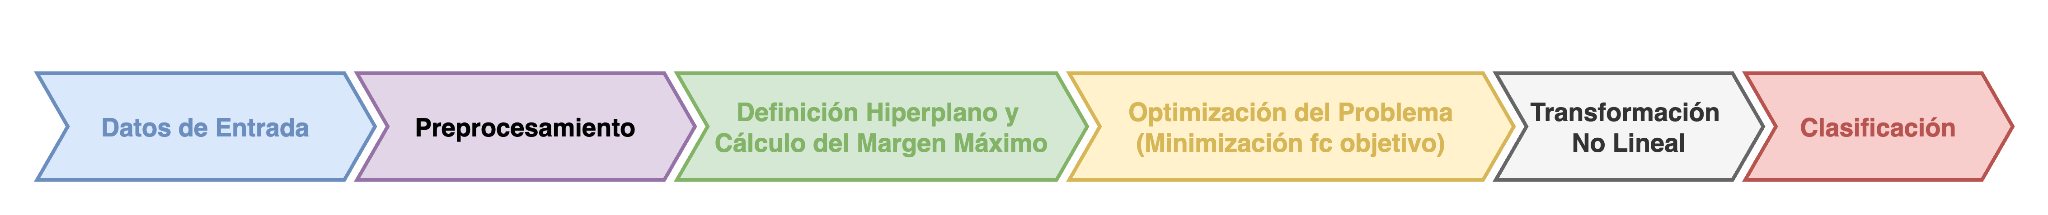
\includegraphics[width=14.33cm,height=1.51cm]{./images/image3.png}
\end{figure}


\begin{center}
\textit{Figura 6. Arquitectura de Flujo del SVM}
\end{center}


El objetivo de la SVM es encontrar el hiperplano que maximiza el margen, formulado como un problema de optimización.

\vspace{1\baselineskip}
\section{Modelo Propuesto: LSTM + Hand landmarker + LLM}

\vspace{1\baselineskip}
En esta sección se describe el modelo a utilizar para probar la hipótesis. A diferencia de los modelos SVM o YOLO-v9e, discutidos en el capítulo 2.1, la red LSTM puede capturar datos históricos de la secuencia de imágenes para poder interpretar señas y gestos de manera dinámica. Para el entrenamiento, se utilizarán datos de hand landmarks derivados del conjunto de datos original, de esta manera se descarta parte del ruido y se sintetiza información relevante.

\vspace{1\baselineskip}
Utilizando este mecanismo se pueden identificar gestos que corresponden a palabras o frases individuales. Al agrupar listas de palabras que forman una oración, el siguiente paso consiste en usarlas como entrada al LLM gpt-3.5-turbo, junto con un prompt que permita obtener una frase con la fluidez propia del lenguaje hablado.

\subsection{Arquitectura del sistema}

\vspace{1\baselineskip}
La arquitectura propuesta está compuesta por tres componentes principales. El primero, una capa de MediaPipe hand landmarker, para obtener la lista de coordenadas de los puntos clave para cada mano.

\vspace{1\baselineskip}
El segundo componente es una red LSTM, que combina capas bidireccionales LSTM y densas para procesar datos secuenciales. La primera capa LSTM bidireccional captura patrones temporales en ambas direcciones y devuelve secuencias completas para la siguiente capa. La segunda LSTM bidireccional resume la información en una representación compacta. Luego, una capa densa con 128 neuronas y activación ReLU permite aprender relaciones no lineales, seguida de un Dropout del 50$\%$ para evitar sobreajuste. Finalmente, una capa densa con activación softmax produce probabilidades para las clases objetivo.

\vspace{1\baselineskip}
El tercer componente consiste en utilizar gpt-3.5-turbo, para derivar oraciones fluidas, dada una lista de palabras, y el prompt ``Convierte la siguiente secuencia de palabras de lengua de señas chilena a una frase en español coherente".

\vspace{2\baselineskip}
\begin{figure}[H]
\centering
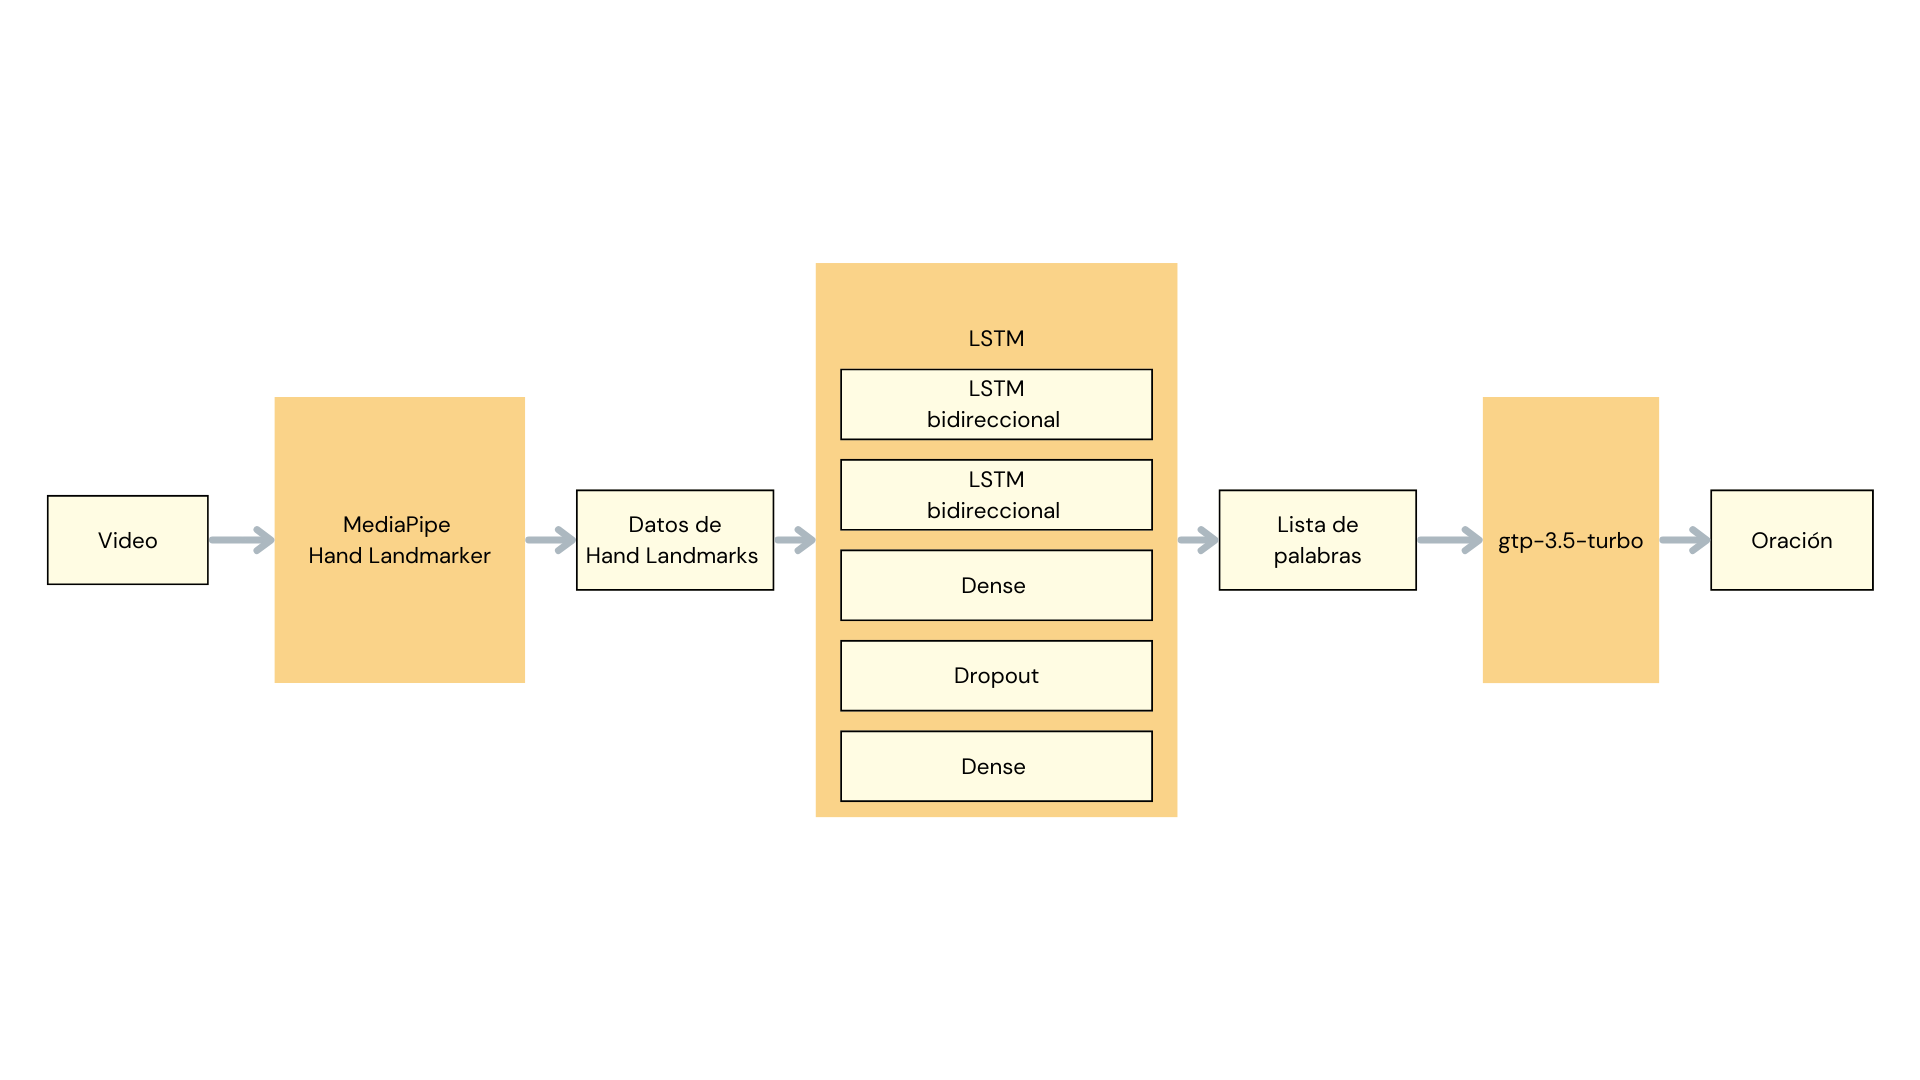
\includegraphics[width=14.33cm,height=4.54cm]{./images/image12.png}
\end{figure}


\vspace{1\baselineskip}
\begin{center}
\textit{Figura 7. Diagrama de bloques de la arquitectura propuesta}
\end{center}


\section{Experimentos}

\vspace{1\baselineskip}
En esta sección se describe el diseño y configuración de los experimentos realizados para validar la hipótesis.

\subsection{Conjunto de datos y configuración de los experimentos}

\subsubsection{Entrenamiento y validación}

\vspace{1\baselineskip}
Para entrenar el modelo, se han elegido 20 etiquetas correspondientes a 20 palabras o frases (una de las etiquetas es ``por favor" que son dos palabras). Estas frases fueron elegidas en base a dos criterios: el primero, por su simplicidad, ya que representan conceptos básicos, y segundo, por su versatilidad, ya que pueden ser permutadas de distintas maneras para obtener oraciones simples.

\vspace{1\baselineskip}
\textbf{Etiquetas elegidas: }por favor, gracias, nombre, yo, tú, bien, sentir, cómo, gustar, ver, hola, permiso, bueno, día, tarde, noche, enamorado, comer, conversar, médico.

\vspace{1\baselineskip}
Como set de datos se han utilizado 50 videos por cada etiqueta, algunos de estos fueron recopilados desde repositorios de dominio público disponibles en la web, y otros fueron capturados de forma propia con una cámara. Para su captura, se grabaron con distintos participantes, y con distintas condiciones de iluminación para evitar el sobreajuste. 

La razón por la que se recopilaron los datos de esta forma es debido a la falta de disponibilidad de un dataset completo y especializado para la lengua de señas chilena.  Esta muestra dista de ser ideal, ya que no es muy extensa, sin embargo se procedió a utilizar data augmentation, introduciendo variaciones en las coordenadas de los hand landmarks, como rotación y traslación para triplicar la cantidad de datos de entrenamiento.

\vspace{1\baselineskip}
Las métricas seleccionadas en los experimentos para medir el rendimiento de los modelos son: tasa de acierto, para las etiquetas individuales, la distancia de Levenshtein (dividida entre la longitud de la oración) para comparar la oración final obtenida, con la oración esperada, y la latencia o tiempo de respuesta entre el cliente y el servidor.

\subsubsection{Configuración de experimentos}

\vspace{1\baselineskip}
\textbf{Diseño: }Para construir el algoritmo se utilizó Python como lenguaje y para el diseño de la arquitectura de la red neuronal. Como plataforma de desarrollo se utilizó Visual Studio Code.

El código es ejecutado en instancia de Google Cloud Platform con una GPU Nvidia T4 con 15 GB de RAM.

\vspace{1\baselineskip}
\textbf{Datasets: }dataset de elaboración propia  conformado por 1.000 videos en formato mp4, con una resolución de 640x480. 50 videos por cada etiqueta.

\vspace{1\baselineskip}
Se realizaron tres tipos de experimento: 

\subsubsection{Entrenamiento y pruebas del modelo LSTM + Hand Landmarks}

Se procede a capturar hand landmarks para cada video y a utilizar estos datos para entrenar el modelo LSTM. Los datos son divididos en 80$\%$ para entrenamiento y 20$\%$ para pruebas. Se define una función de pérdida categórica y una métrica de precisión para evaluar el rendimiento. El entrenamiento usa un callback de EarlyStopping para detenerse si la pérdida de validación deja de mejorar durante 10 épocas, lo que previene el sobreentrenamiento. 

\vspace{1\baselineskip}
A continuación se prueban distintos hiperparámetros, para evaluar el desempeño, en base a la tasa de acierto respecto a los datos de prueba.

\vspace{1\baselineskip}
\subsubsection{Pruebas de LLMs}

Se probaron diferentes modelos de lenguaje de gran escala para comparar el resultado obtenido con la oración esperada, utilizando la distancia de Levenshtein, dividida entre la longitud de la oración esperada, y así obtener el porcentaje de coincidencia.

\vspace{2\baselineskip}
\( P  =  (1 -levenshtein(E, A) / max(len(E), len(A)) \ast  100\)

\vspace{2\baselineskip}
Donde \textit{E} es la oración esperada, \textit{A }es la oración obtenida por el LLM, \( levenshtein\) es la función de distancia de Levenshtein, \( \max\) es la función de máximo, y \( len\) es la longitud de la cadena de texto.

\vspace{1\baselineskip}
Como métrica secundaria a evaluar, está el tiempo de respuesta, medido en milisegundos, de forma que se consiga un balance entre precisión y velocidad.

\vspace{1\baselineskip}
Para llevar a cabo este experimento, se utilizó el \textit{Playground }de openai, y también la herramienta groqcloud, ambas opciones consisten en una interfaz web, que permite introducir prompts al modelo de lenguaje, y visualizar la salida obtenida, junto con el tiempo de respuesta.

\vspace{1\baselineskip}
\subsubsection{Integración y latencia Cliente-Servidor}

Se implementó un prototipo del intercambio de datos entre el cliente y el servidor, ejecutando un sitio web implementado con Javascript/React, ejecutado en el navegador Google Chrome para enviar la secuencia de imágenes capturadas por la webcam, correspondiente a la seña para la palabra ``gracias" via WebSockets, de manera que puedan ser procesadas en el servidor y retornar como respuesta al cliente la oración resultante de ejecutar los componentes presentados en el punto 4.1 sobre dicha secuencia de imágenes.

\vspace{1\baselineskip}
La métrica a considerar es la latencia, definida como el tiempo en milisegundos, transcurrido desde que se empieza a enviar la última imagen de la secuencia hasta que llega la respuesta al cliente. Para este experimento se simulan diferentes velocidades de conexión utilizando las herramientas para desarrolladores de Google Chrome.

\vspace{1\baselineskip}
Para ejecutar este experimento de forma automatizada, se utiliza un script de automatización de navegador utilizando la librería puppeteer, para poder ejecutar 1000 iteraciones.

\begin{figure}[H]
\centering
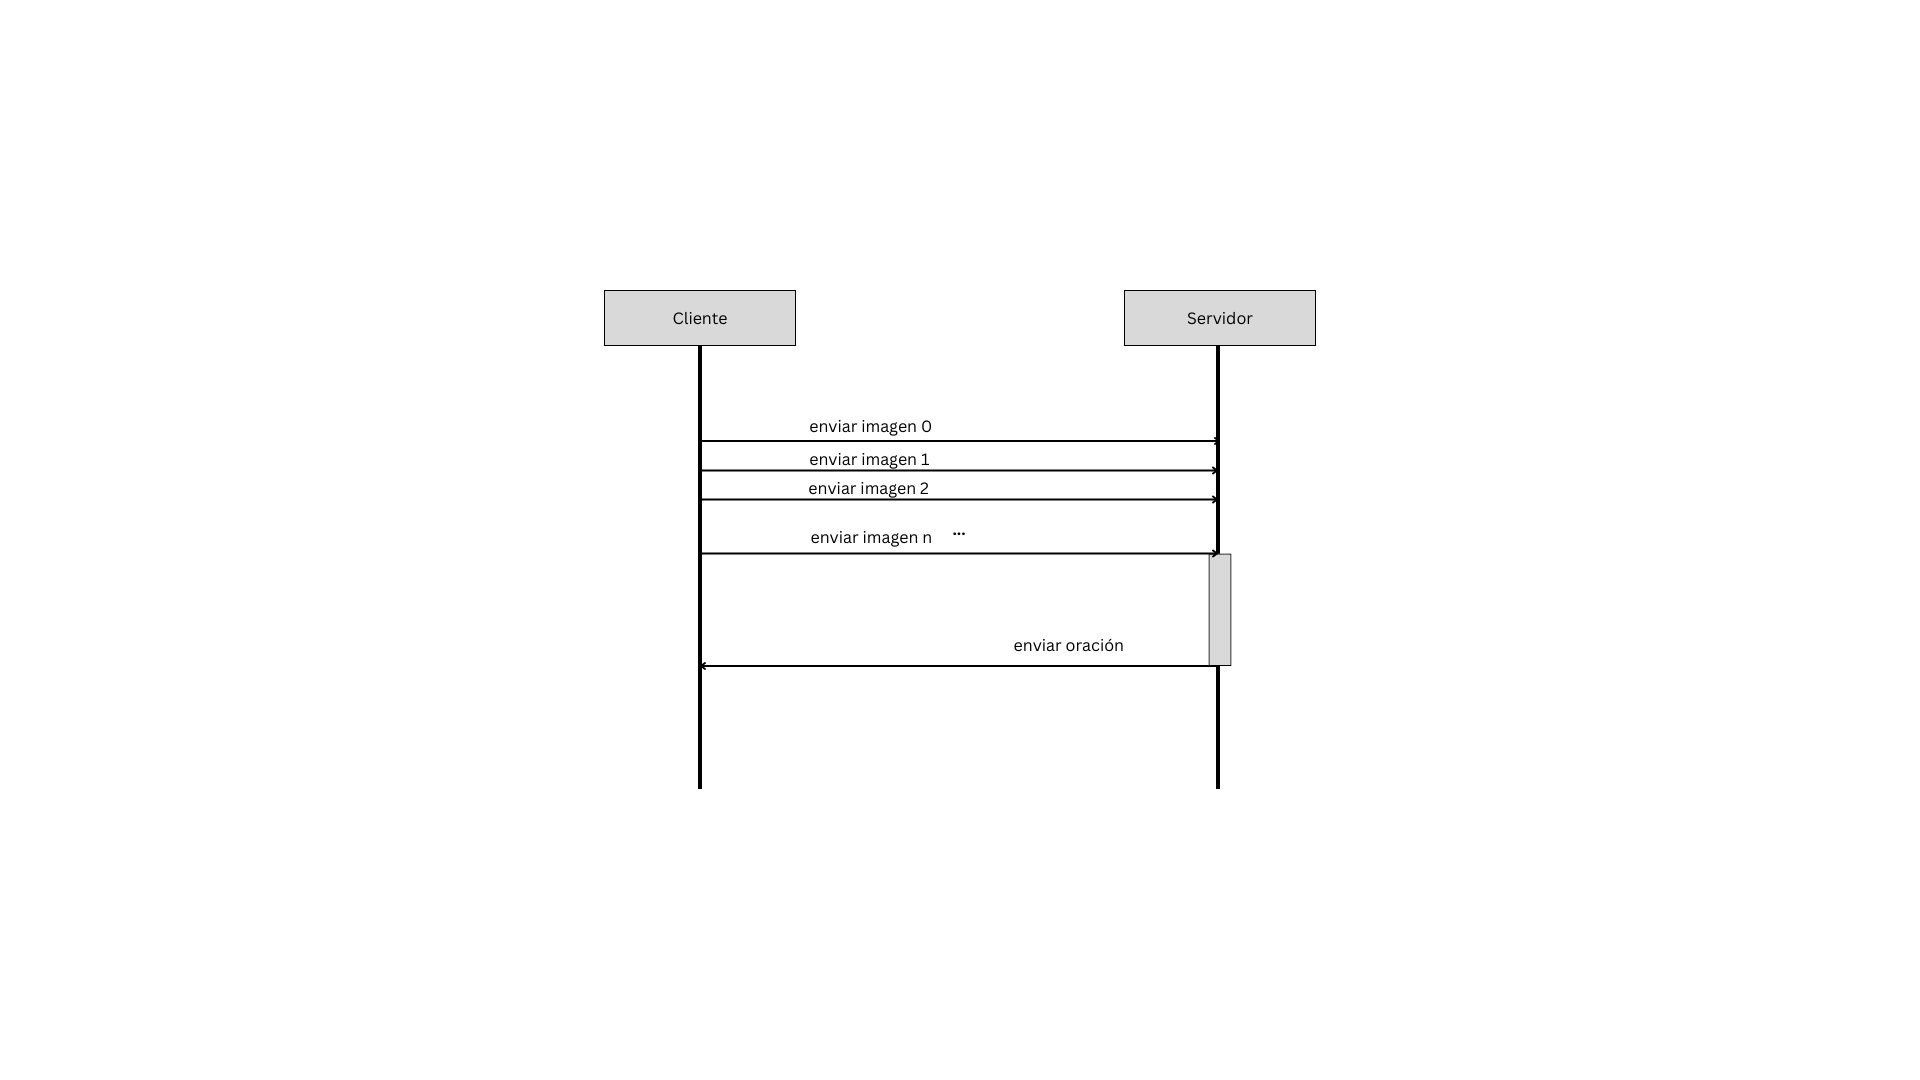
\includegraphics[width=11.06cm,height=7.59cm]{./images/image10.png}
\end{figure}


\begin{center}
\textit{Figura 8. Diagrama de secuencia cliente-servidor}
\end{center}


\vspace{1\baselineskip}
\subsubsection{Comparación de costos}

Finalmente, se evalúan los costos de implementación del sistema, para comparar con el costo por hora de contratar un intérprete profesional de señas.

\section{Resultados}

\vspace{1\baselineskip}
En esta sección se presentan los resultados para cada experimento.

\subsection{Hand Landmarks + Modelo LSTM}

\vspace{1\baselineskip}
En la siguiente tabla se presenta la tasa de acierto para las combinaciones de hiperparámetros consideradas:

\begin{table}[H]
\begin{adjustbox}{max width=\textwidth}
\begin{tabular}{p{4.13cm}p{4.13cm}p{4.13cm}p{4.13cm}p{4.13cm}p{4.13cm}p{4.13cm}p{4.13cm}}
\hline
\multicolumn{1}{|p{4.13cm}}{Epochs} & 
\multicolumn{1}{|p{4.13cm}}{Número de unidades por capa LSTM} & 
\multicolumn{1}{|p{4.13cm}}{Función de activación} & 
\multicolumn{1}{|p{4.13cm}|}{Tasa de acierto} \\ 
\hline
\multicolumn{1}{|p{4.13cm}}{50} & 
\multicolumn{1}{|p{4.13cm}}{64} & 
\multicolumn{1}{|p{4.13cm}}{relu} & 
\multicolumn{1}{|p{4.13cm}|}{0.83} \\ 
\hline
\multicolumn{1}{|p{4.13cm}}{50} & 
\multicolumn{1}{|p{4.13cm}}{64} & 
\multicolumn{1}{|p{4.13cm}}{tanh} & 
\multicolumn{1}{|p{4.13cm}|}{0.61} \\ 
\hline
\multicolumn{1}{|p{4.13cm}}{50} & 
\multicolumn{1}{|p{4.13cm}}{128} & 
\multicolumn{1}{|p{4.13cm}}{relu} & 
\multicolumn{1}{|p{4.13cm}|}{0.43} \\ 
\hline
\multicolumn{1}{|p{4.13cm}}{100} & 
\multicolumn{1}{|p{4.13cm}}{64} & 
\multicolumn{1}{|p{4.13cm}}{relu} & 
\multicolumn{1}{|p{4.13cm}|}{0.91} \\ 
\hline
\multicolumn{1}{|p{4.13cm}}{100} & 
\multicolumn{1}{|p{4.13cm}}{128} & 
\multicolumn{1}{|p{4.13cm}}{relu} & 
\multicolumn{1}{|p{4.13cm}|}{0.84} \\ 
\hline
\end{tabular}
\end{adjustbox}
\end{table}
\vspace{2\baselineskip}
\begin{center}
\textit{Tabla 1. Resultados del modelo propuesto con diferentes hiperparámetros}
\end{center}


\vspace{2\baselineskip}
La configuración que obtuvo una mejor tasa de acierto es: 100 epochs, 64 unidades por capa y función relu.

\vspace{1\baselineskip}
\begin{figure}[H]
\centering
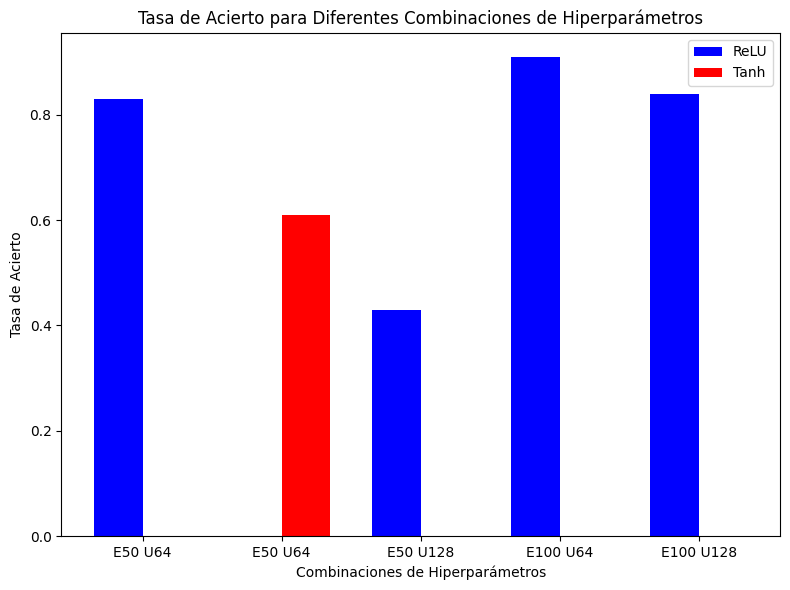
\includegraphics[width=12.82cm,height=9.61cm]{./images/image11.png}
\end{figure}


\vspace{1\baselineskip}
\begin{center}
Figura 9. Tasa de acierto para diferentes combinaciones de hiperparámetros
\end{center}

\vspace{3\baselineskip}

\subsection{LLMs}

Se evalúan tres modelos de lenguaje: gpt-4o-mini, gpt-3.5-turbo de OpenAI y llama-3.1-8b-instant de Meta. Elegidos por considerar que tienen un balance adecuado entre velocidad y precisión. A continuación se presentan los resultados obtenidos para cada experimento, y la comparación de las métricas.

Prompt: ``Convierte la siguiente secuencia de palabras de lengua de señas chilena a una frase en español coherente: <secuencia>"

\vspace{1\baselineskip}

\newpage

gpt-4o-mini:

\begin{table}[H]
\begin{adjustbox}{max width=\textwidth}
\begin{tabular}{p{3.44cm}p{4.02cm}p{3.92cm}p{2.35cm}p{2.78cm}p{3.44cm}p{4.02cm}p{3.92cm}p{2.35cm}p{2.78cm}}
\hline
\multicolumn{1}{|p{3.44cm}}{Secuencia} & 
\multicolumn{1}{|p{4.02cm}}{\raggedright
\textcolor[HTML]{434343}{Respuesta esperada}} & 
\multicolumn{1}{|p{3.92cm}}{\textcolor[HTML]{434343}{Respuesta obtenida}} & 
\multicolumn{1}{|p{2.35cm}}{\raggedright
{\small \textcolor[HTML]{434343}{$\%$ de coincidencia}}} & 
\multicolumn{1}{|p{2.78cm}|}{\raggedright
{\small \textcolor[HTML]{434343}{Tiempo de respuesta (ms)}}} \\ 
\hline
\multicolumn{1}{|p{3.44cm}}{yo, gustar,conversar, médico} & 
\multicolumn{1}{|p{4.02cm}}{Me gusta conversar con el médico} & 
\multicolumn{1}{|p{3.92cm}}{Me gusta conversar con el médico} & 
\multicolumn{1}{|p{2.35cm}}{\raggedleft
100.00} & 
\multicolumn{1}{|p{2.78cm}|}{\raggedleft
1426.00} \\ 
\hline
\multicolumn{1}{|p{3.44cm}}{bueno, día} & 
\multicolumn{1}{|p{4.02cm}}{Buenos días} & 
\multicolumn{1}{|p{3.92cm}}{Buen día} & 
\multicolumn{1}{|p{2.35cm}}{\raggedleft
63.64} & 
\multicolumn{1}{|p{2.78cm}|}{\raggedleft
535.00} \\ 
\hline
\multicolumn{1}{|p{3.44cm}}{bueno, noche} & 
\multicolumn{1}{|p{4.02cm}}{buenas noches} & 
\multicolumn{1}{|p{3.92cm}}{Buena noche} & 
\multicolumn{1}{|p{2.35cm}}{\raggedleft
84.62} & 
\multicolumn{1}{|p{2.78cm}|}{\raggedleft
531.00} \\ 
\hline
\multicolumn{1}{|p{3.44cm}}{yo sentir bien} & 
\multicolumn{1}{|p{4.02cm}}{me siento bien} & 
\multicolumn{1}{|p{3.92cm}}{Yo me siento bien} & 
\multicolumn{1}{|p{2.35cm}}{\raggedleft
82.35} & 
\multicolumn{1}{|p{2.78cm}|}{\raggedleft
752.00} \\ 
\hline
\multicolumn{1}{|p{3.44cm}}{yo gustar comer} & 
\multicolumn{1}{|p{4.02cm}}{me gusta comer} & 
\multicolumn{1}{|p{3.92cm}}{A mí me gusta comer} & 
\multicolumn{1}{|p{2.35cm}}{\raggedleft
73.68} & 
\multicolumn{1}{|p{2.78cm}|}{\raggedleft
642.00} \\ 
\hline
\multicolumn{1}{|p{3.44cm}}{bueno, día; tú, cómo, nombre} & 
\multicolumn{1}{|p{4.02cm}}{buenos días, cómo te llamas} & 
\multicolumn{1}{|p{3.92cm}}{Buen día. ¿Cómo te llamas?} & 
\multicolumn{1}{|p{2.35cm}}{\raggedleft
77.78} & 
\multicolumn{1}{|p{2.78cm}|}{\raggedleft
723.00} \\ 
\hline
\multicolumn{1}{|p{3.44cm}}{} & 
\multicolumn{1}{|p{4.02cm}}{} & 
\multicolumn{1}{|p{3.92cm}}{Promedio} & 
\multicolumn{1}{|p{2.35cm}}{\raggedleft
80.34} & 
\multicolumn{1}{|p{2.78cm}|}{\raggedleft
768.17} \\ 
\hline
\end{tabular}
\end{adjustbox}
\end{table}
\vspace{4\baselineskip}
\begin{center}
\textit{Tabla 2. Resultados de las pruebas con gpt-4o-mini}
\end{center}


\vspace{2\baselineskip}
gpt-3.5-turbo:

\begin{table}[H]
\begin{adjustbox}{max width=\textwidth}
\begin{tabular}{p{3.44cm}p{4.02cm}p{3.92cm}p{2.35cm}p{2.78cm}p{3.44cm}p{4.02cm}p{3.92cm}p{2.35cm}p{2.78cm}}
\hline
\multicolumn{1}{|p{3.44cm}}{Secuencia} & 
\multicolumn{1}{|p{4.02cm}}{\textcolor[HTML]{434343}{Respuesta esperada}} & 
\multicolumn{1}{|p{3.92cm}}{\textcolor[HTML]{434343}{Respuesta obtenida}} & 
\multicolumn{1}{|p{2.35cm}}{{\small \textcolor[HTML]{434343}{$\%$ de coincidencia}}} & 
\multicolumn{1}{|p{2.78cm}|}{{\small \textcolor[HTML]{434343}{Tiempo de respuesta (ms)}}} \\ 
\hline
\multicolumn{1}{|p{3.44cm}}{yo, gustar,conversar, médico} & 
\multicolumn{1}{|p{4.02cm}}{Me gusta conversar con el médico} & 
\multicolumn{1}{|p{3.92cm}}{Me gusta hablar con el médico} & 
\multicolumn{1}{|p{2.35cm}}{\raggedleft
78.13} & 
\multicolumn{1}{|p{2.78cm}|}{\raggedleft
716} \\ 
\hline
\multicolumn{1}{|p{3.44cm}}{bueno, día} & 
\multicolumn{1}{|p{4.02cm}}{Buenos días} & 
\multicolumn{1}{|p{3.92cm}}{Buenos días} & 
\multicolumn{1}{|p{2.35cm}}{\raggedleft
100.00} & 
\multicolumn{1}{|p{2.78cm}|}{\raggedleft
746} \\ 
\hline
\multicolumn{1}{|p{3.44cm}}{bueno, noche} & 
\multicolumn{1}{|p{4.02cm}}{buenas noches} & 
\multicolumn{1}{|p{3.92cm}}{Buenas noches} & 
\multicolumn{1}{|p{2.35cm}}{\raggedleft
100.00} & 
\multicolumn{1}{|p{2.78cm}|}{\raggedleft
758} \\ 
\hline
\multicolumn{1}{|p{3.44cm}}{yo sentir bien} & 
\multicolumn{1}{|p{4.02cm}}{me siento bien} & 
\multicolumn{1}{|p{3.92cm}}{Me siento bien} & 
\multicolumn{1}{|p{2.35cm}}{\raggedleft
100.00} & 
\multicolumn{1}{|p{2.78cm}|}{\raggedleft
733} \\ 
\hline
\multicolumn{1}{|p{3.44cm}}{yo gustar comer} & 
\multicolumn{1}{|p{4.02cm}}{me gusta comer} & 
\multicolumn{1}{|p{3.92cm}}{Me gusta comer} & 
\multicolumn{1}{|p{2.35cm}}{\raggedleft
100.00} & 
\multicolumn{1}{|p{2.78cm}|}{\raggedleft
632} \\ 
\hline
\multicolumn{1}{|p{3.44cm}}{bueno, día, tú, cómo, nombre} & 
\multicolumn{1}{|p{4.02cm}}{buenos días, cómo te llamas} & 
\multicolumn{1}{|p{3.92cm}}{Buenos días, ¿cómo te llamas?} & 
\multicolumn{1}{|p{2.35cm}}{\raggedleft
100.00} & 
\multicolumn{1}{|p{2.78cm}|}{\raggedleft
833} \\ 
\hline
\multicolumn{1}{|p{3.44cm}}{} & 
\multicolumn{1}{|p{4.02cm}}{} & 
\multicolumn{1}{|p{3.92cm}}{Promedio} & 
\multicolumn{1}{|p{2.35cm}}{\raggedleft
96.35} & 
\multicolumn{1}{|p{2.78cm}|}{\raggedleft
736.33} \\ 
\hline
\end{tabular}
\end{adjustbox}
\end{table}
\vspace{1\baselineskip}
\begin{center}
\textit{Tabla 3. Resultados de las pruebas con gpt-3.5-turbo}
\end{center}


\vspace{3\baselineskip}
llama-3.1-8b-instant:

\begin{table}[H]
\begin{adjustbox}{max width=\textwidth}
\begin{tabular}{p{3.44cm}p{4.02cm}p{4.6cm}p{1.67cm}p{2.78cm}p{3.44cm}p{4.02cm}p{4.6cm}p{1.67cm}p{2.78cm}}
\hline
\multicolumn{1}{|p{3.44cm}}{Secuencia} & 
\multicolumn{1}{|p{4.02cm}}{\textcolor[HTML]{434343}{Respuesta esperada}} & 
\multicolumn{1}{|p{4.6cm}}{\textcolor[HTML]{434343}{Respuesta obtenida}} & 
\multicolumn{1}{|p{1.67cm}}{\textcolor[HTML]{434343}{$\%$ de coinci-} \newline
\textcolor[HTML]{434343}{dencia}} & 
\multicolumn{1}{|p{2.78cm}|}{\textcolor[HTML]{434343}{Tiempo de respuesta (ms)}} \\ 
\hline
\multicolumn{1}{|p{3.44cm}}{yo, gustar,conversar, médico} & 
\multicolumn{1}{|p{4.02cm}}{Me gusta conversar con el médico} & 
\multicolumn{1}{|p{4.6cm}}{Me gustaría conversar con un médico} & 
\multicolumn{1}{|p{1.67cm}}{\raggedleft
85.71} & 
\multicolumn{1}{|p{2.78cm}|}{\raggedleft
124.00} \\ 
\hline
\multicolumn{1}{|p{3.44cm}}{bueno, día} & 
\multicolumn{1}{|p{4.02cm}}{Buenos días} & 
\multicolumn{1}{|p{4.6cm}}{Hoy es un buen día} & 
\multicolumn{1}{|p{1.67cm}}{\raggedleft
27.78} & 
\multicolumn{1}{|p{2.78cm}|}{\raggedleft
113.00} \\ 
\hline
\multicolumn{1}{|p{3.44cm}}{bueno, noche} & 
\multicolumn{1}{|p{4.02cm}}{buenas noches} & 
\multicolumn{1}{|p{4.6cm}}{La noche está bien} & 
\multicolumn{1}{|p{1.67cm}}{\raggedleft
22.22} & 
\multicolumn{1}{|p{2.78cm}|}{\raggedleft
221.00} \\ 
\hline
\multicolumn{1}{|p{3.44cm}}{yo sentir bien} & 
\multicolumn{1}{|p{4.02cm}}{me siento bien} & 
\multicolumn{1}{|p{4.6cm}}{Me siento bien} & 
\multicolumn{1}{|p{1.67cm}}{\raggedleft
100.00} & 
\multicolumn{1}{|p{2.78cm}|}{\raggedleft
124.00} \\ 
\hline
\multicolumn{1}{|p{3.44cm}}{yo gustar comer} & 
\multicolumn{1}{|p{4.02cm}}{me gusta comer} & 
\multicolumn{1}{|p{4.6cm}}{Me gusta comer} & 
\multicolumn{1}{|p{1.67cm}}{\raggedleft
100.00} & 
\multicolumn{1}{|p{2.78cm}|}{\raggedleft
147.00} \\ 
\hline
\multicolumn{1}{|p{3.44cm}}{bueno, día, tú, cómo, nombre} & 
\multicolumn{1}{|p{4.02cm}}{buenos días, cómo te llamas} & 
\multicolumn{1}{|p{4.6cm}}{¿Cómo te llamas? (Qué bueno que seas un buen día, ¿tu nombre es...?)} & 
\multicolumn{1}{|p{1.67cm}}{\raggedleft
21.219} & 
\multicolumn{1}{|p{2.78cm}|}{\raggedleft
160} \\ 
\hline
\multicolumn{1}{|p{3.44cm}}{} & 
\multicolumn{1}{|p{4.02cm}}{} & 
\multicolumn{1}{|p{4.6cm}}{Promedio} & 
\multicolumn{1}{|p{1.67cm}}{\raggedleft
59.49} & 
\multicolumn{1}{|p{2.78cm}|}{\raggedleft
148.17} \\ 
\hline
\end{tabular}
\end{adjustbox}
\end{table}
\vspace{1\baselineskip}
\begin{center}
\textit{Tabla 4. Resultados de las pruebas con }llama-3.1-8b-instant 
\end{center}


\vspace{2\baselineskip}
Al comparar estos tres modelos, gpt-3.5-turbo obtiene un porcentaje de precisión significativamente mayor, por otro lado llama-3.1-8b-instant arroja los mejores tiempos de respuesta, pero el porcentaje de coincidencia es inferior. Se puede concluir que el mejor modelo de los tres para esta tarea es gpt-3.5-turbo, al presentar el mejor balance precisión/velocidad.

\vspace{2\baselineskip}
\begin{figure}[H]
\centering
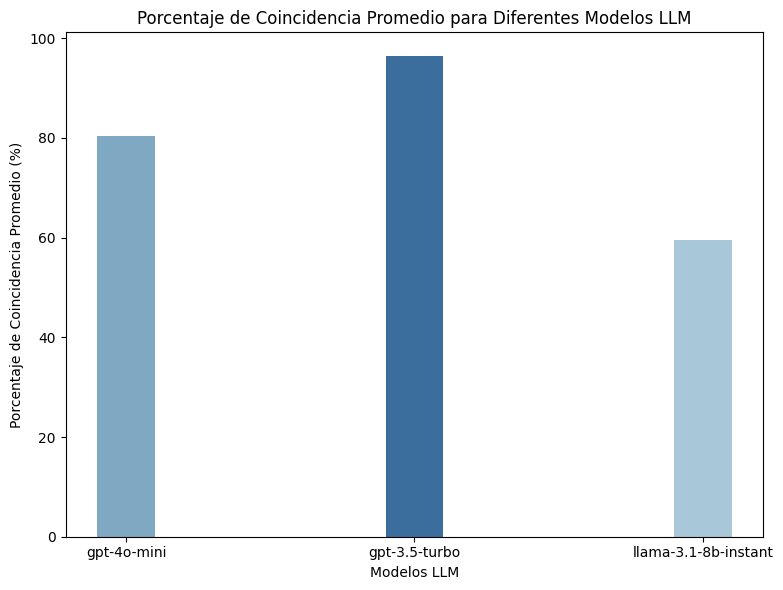
\includegraphics[width=12.58cm,height=9.5cm]{./images/image7.png}
\end{figure}


\begin{center}
\textit{Figura 10. Porcentaje de coincidencia promedio para los diferentes modelos LLM}
\end{center}


\vspace{1\baselineskip}
\textit{\begin{figure}[H]
\centering
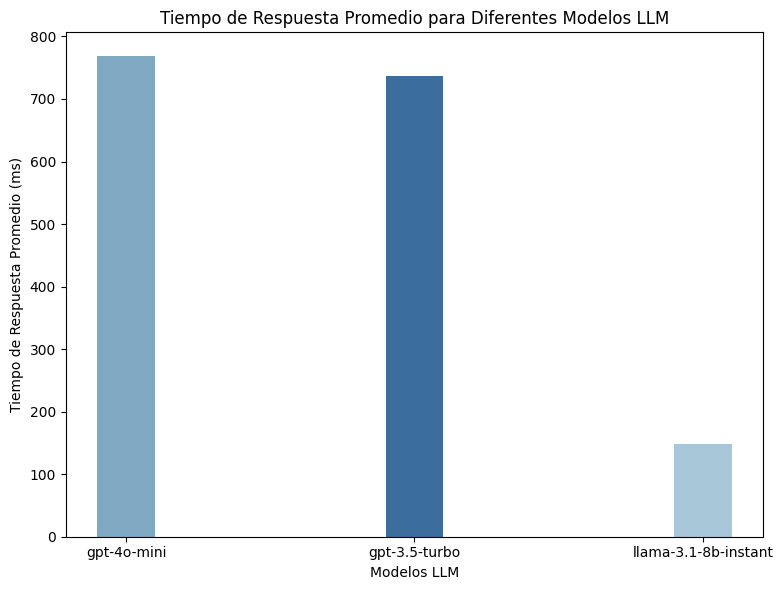
\includegraphics[width=12.73cm,height=9.61cm]{./images/image8.png}
\end{figure}
}

\vspace{1\baselineskip}
\begin{center}
\textit{Figura 11. Tiempo de Respuesta Promedio para Diferentes Modelos LLM}
\end{center}


\vspace{2\baselineskip}
\subsection{Integración y latencia cliente-servidor}

Al simular diferentes velocidades en conexión, en la configuración mencionada en 5.1.2.3,  haciendo 1000 iteraciones, se obtienen los siguientes resultados:

\begin{table}[H]
\begin{adjustbox}{max width=\textwidth}
\begin{tabular}{p{4.13cm}p{4.13cm}p{4.13cm}p{4.13cm}p{4.13cm}p{4.13cm}p{4.13cm}p{4.13cm}}
\hline
\multicolumn{1}{|p{4.13cm}}{\raggedright
Nombre preset} & 
\multicolumn{1}{|p{4.13cm}}{\raggedright
Velocidad de subida} & 
\multicolumn{1}{|p{4.13cm}}{\raggedright
Velocidad de bajada} & 
\multicolumn{1}{|p{4.13cm}|}{\raggedright
Tiempo de respuesta promedio (ms)} \\ 
\hline
\multicolumn{1}{|p{4.13cm}}{\raggedright
4g rápido} & 
\multicolumn{1}{|p{4.13cm}}{\textcolor[HTML]{0C0D0E}{400 Kbit/s}} & 
\multicolumn{1}{|p{4.13cm}}{\textcolor[HTML]{0C0D0E}{8.10 Mb/s}} & 
\multicolumn{1}{|p{4.13cm}|}{\raggedright
945.75} \\ 
\hline
\multicolumn{1}{|p{4.13cm}}{\raggedright
4G lento} & 
\multicolumn{1}{|p{4.13cm}}{\textcolor[HTML]{0C0D0E}{675 Kb/s}} & 
\multicolumn{1}{|p{4.13cm}}{\textcolor[HTML]{0C0D0E}{1.44 Mb/s}} & 
\multicolumn{1}{|p{4.13cm}|}{\raggedright
1600.40} \\ 
\hline
\multicolumn{1}{|p{4.13cm}}{\raggedright
3G} & 
\multicolumn{1}{|p{4.13cm}}{\textcolor[HTML]{0C0D0E}{1.35 Mb/s}} & 
\multicolumn{1}{|p{4.13cm}}{\textcolor[HTML]{0C0D0E}{400 Kbit/s}} & 
\multicolumn{1}{|p{4.13cm}|}{\raggedright
2150.20} \\ 
\hline
\end{tabular}
\end{adjustbox}
\end{table}
\vspace{2\baselineskip}
\begin{center}
\textit{Tabla 5. Resultados de las pruebas de latencia cliente-servidor}
\end{center}


\vspace{2\baselineskip}
Podemos observar que el orden de magnitud de las respuestas con el sistema actual, a grandes rasgos, se encuentra en el orden de los 1 a 2 segundos.

\vspace{1\baselineskip}
\subsection{Evaluación de costos del sistema}

\subsubsection{Costos del sistema}

\vspace{1\baselineskip}
Se toman como referencia los costos con el proveedor de cloud computing Amazon AWS, y un

valor del dólar de CLP 970. También se toma en cuenta el costo de un equipo de tres desarrolladores trabajando a tiempo completo para proveer soporte y mejoras continuas al sistema, con precios promedio de mercado para 2024.

\vspace{1\baselineskip}
Se desestiman en este caso los costos por hora de los dispositivos a utilizar como laptop o

dispositivos móviles, ya que asumimos que los mismos se encuentran disponibles en un

consultorio, y no estaríamos incurriendo en costos adicionales.

\begin{table}[H]
\begin{adjustbox}{max width=\textwidth}
\begin{tabular}{p{4.21cm}p{6.8cm}p{5.5cm}p{4.21cm}p{6.8cm}p{5.5cm}}
\hline
\multicolumn{1}{|p{4.21cm}}{Item} & 
\multicolumn{1}{|p{6.8cm}}{Detalles} & 
\multicolumn{1}{|p{5.5cm}|}{Costo por hora CLP} \\ 
\hline
\multicolumn{1}{|p{4.21cm}}{Servidor} & 
\multicolumn{1}{|p{6.8cm}}{Instancia g5.xlarge Amazon aws} & 
\multicolumn{1}{|p{5.5cm}|}{975,82} \\ 
\hline
\multicolumn{1}{|p{4.21cm}}{Otros costos de infraestructura} & 
\multicolumn{1}{|p{6.8cm}}{Almacenamiento, Tráfico de red, \newline
Logging, API gateway.} & 
\multicolumn{1}{|p{5.5cm}|}{970} \\ 
\hline
\multicolumn{1}{|p{4.21cm}}{Costos de soporte / mejora \newline
contínua \newline
} & 
\multicolumn{1}{|p{6.8cm}}{Equipo de 3 desarrolladores } & 
\multicolumn{1}{|p{5.5cm}|}{60.000} \\ 
\hline
\multicolumn{1}{|p{4.21cm}}{} & 
\multicolumn{1}{|p{6.8cm}}{Total} & 
\multicolumn{1}{|p{5.5cm}|}{\textbf{61.945}} \\ 
\hline
\end{tabular}
\end{adjustbox}
\end{table}
\vspace{1\baselineskip}
\begin{center}
\textit{Tabla 6. Desglose de costos de implementación del sistema}
\end{center}


\vspace{1\baselineskip}
\subsubsection{Comparación con el costo de intérprete profesional}

\vspace{1\baselineskip}
Después de una investigación de los valores del mercado en Santiago de Chile, se obtuvo un costo promedio de 20.000 pesos/hora para contratar un intérprete de señas. Sin incluir los costos de transporte para acudir al lugar.

\vspace{1\baselineskip}
El costo de referencia del punto 6.4.1 es mayor al costo de un intérprete, si fuese utilizado por una sóla persona, pero tomando en cuenta que con esta configuración el sistema tiene la capacidad de atender cientos de peticiones de manera concurrente, podemos determinar que el costo es órdenes de magnitud menor que el del intérprete profesional.

\vspace{1\baselineskip}
\newpage
\section{Conclusiones}

\vspace{1\baselineskip}
En el presente trabajo se ha realizado una revisión del estado del arte de los métodos para interpretar la Lengua de señas Chilena, así como otros métodos utilizados internacionalmente, proponiendo una solución que combina diferentes modelos para obtener un resultado con una tasa de acierto y porcentaje de coincidencia de las traducciones finales, sobre 90$\%$, en el contexto de una arquitectura cliente-servidor que permita su ejecución desde dispositivos portátiles, en particular de baja y media gama, con una latencia en el orden de los 1 a 2 segundos.

\vspace{1\baselineskip}
De estos resultados podemos concluir que este esquema tiene potencial para permitir la accesibilidad de las personas sordas a los servicios de salud, sin necesidad de un intérprete. Sin embargo, aún quedan grandes retos por resolver. Por un lado, es necesario recopilar un conjunto de datos robusto y representativo de la Lengua de Señas Chilena, ya que los datos actuales son muy limitados y no abarcan la diversidad de señas necesarias para aplicaciones generalizadas. Por otro lado, reducir la latencia a menos de un segundo, mejoraría significativamente la calidad de la comunicación, permitiendo interacciones más fluidas.

\vspace{3\baselineskip}
\section{Bibliografía}

\vspace{1\baselineskip}
[1] Herrera, M. (2023, Febrero) Falta de inclusión, estigma social y discriminación: la compleja realidad diaria que vive una persona sorda en Chile. La Tercera. Santiago. p. 1

\vspace{1\baselineskip}
[2] Mendía R. y García C. (2021, Enero). Comunidad sorda y salud mental: Un abandono silencioso. La Tercera. Santiago. p. 1

\vspace{1\baselineskip}
[3] Gonzalez, C. y Yimes F. (2016) Sistema de reconocimiento gestual de lengua de señas chilena mediante cámara digital p. 36-41

\vspace{1\baselineskip}
[4] Acuña, X., Adamo, D. y Cabrera I. (2009) Diccionario Bilingüe de Lengua de Señas Chilena-Español. p. 17-18

\vspace{1\baselineskip}
[5] Andrare, L. y Catril, R. (2022) Reconocimiento en tiempo real del alfabeto de lengua de señas chilena empleando aprendizaje automático. p. 53-62

\vspace{1\baselineskip}
[6] Pathan, R. K., Biswas, M., Yasmin, S., Khandaker, M. U., Salman, M., $\&$ Youssef, A. A. F. (2023). Sign language recognition using the fusion of image and hand landmarks through multi-headed convolutional neural network. p. 4-9

\vspace{1\baselineskip}
[7] Bala, D., Sarkar, B., Abdullah, M. I., $\&$ Hossain, M. A. (2021). American Sign Language alphabets recognition using convolutional neural network. International Journal of Knowledge Based Computer Systems.

\vspace{1\baselineskip}
[8] Makkar, A., Makkar, D., Patel, A., $\&$ Hebert, L. (2024). SignSpeak: Open-source time series classification for ASL translation.

\vspace{1\baselineskip}
[9] Renjith, S., $\&$ Manazhy, R. (2024). Sign language: A systematic review on classification and recognition. P. 14-15

\vspace{1\baselineskip}
[10] Gong, J., Foo, L. G., He, Y., Rahmani, H., $\&$ Liu, J. (2024). LLMs are good sign language translators. 

[11] Imran, A., Hulikal, M. S., $\&$ Gardi, H. A. A. (2024). Real Time American Sign Language Detection Using YOLO-v9

[12] Ministerio de Desarrollo Social y Servicio Nacional de la Discapacidad (SENADIS). (2015). II Estudio Nacional de la Discapacidad.


\end{document}